% !TEX spellcheck = en_US

% ~~~~~~~~~~~~~~~~~~~~~~~~~~~~~~~~~~~~~~ V
% (NC) 2021 Haluk Bingol
% github.com/halukbingol/LaTeX-Templates
%
% Licensees may copy, distribute, display, and perform the work and make derivative works 
% and remixes based on it only for non-commercial purposes. 
% ~~~~~~~~~~~~~~~~~~~~~~~~~~~~~~~~~~~~~~ A




\documentclass[10pt,journal,compsoc]{IEEEtran}
%\documentclass[pre,twocolumn,showkeys,longbibliography]{revtex4-1}
%\documentclass[pre,twocolumn,showkeys,longbibliography,nofootinbib]{revtex4-1}
%\documentclass[twocolumn,preprintnumbers,amsmath,amssymb,superscriptaddress,pre]{revtex4}
%\documentclass[10pt,journal,compsoc]{IEEEtran}




%: ~~~~~~~~~~~~~~~~~~~~~~~~~~~~~~~~~~~~~~~ V HB Packages v2020-12-11
	\usepackage[utf8]{inputenc} % To use Unicode characters
	\usepackage[iso]{datetime}
	\newcommand{\hbTimeStamp}{{\color{red}--Draft-- v\today/\currenttime}} % version
	%	\usepackage{etex}
	\usepackage{amssymb}
%	\usepackage{enumitem}
	\usepackage{enumerate}
	
	
	\usepackage[a4paper]{geometry}
	
	\usepackage{xcolor}
	% black, blue, brown, cyan, darkgray, gray, green, lightgray, lime, 
	% magenta, olive, orange, pink, purple, red, teal, violet, white, yellow
		\definecolor{darkred}{rgb}{0.8,0.1,0.1}
		\definecolor{darkgreen}{rgb}{0,0.5,0}
		\definecolor{darkblue}{rgb}{0,0,0.5}
		\colorlet{RED}{red}


	\usepackage[colorlinks=true,linkcolor=red,urlcolor=blue,citecolor=red]%
		{hyperref}
	\usepackage{graphicx,epstopdf}
	% \graphicspath{{fig}}
	\graphicspath{{../common/figures/}}
	% \DeclareGraphicsExtensions{.pdf,.jpeg,.png,.eps}
	% \DeclareGraphicsRule{.tif}{png}{.png}%
	%	{`convert #1 `dirname #1`/`basename #1 .tif`.png}
%	\usepackage{subfigure}
%	\usepackage{subfig}
	\usepackage{subcaption}
% ~~~~~~~~~~~~~~~~~~~~~~~~~~~~~~~~~~~~~~~ A




%: ~~~~~~~~~~~~~~~~~~~~~~~~~~~~~~~~~~~~~~~ V HB Common Declarations v20200421
%	\newcommand{\hbTimeStamp}{{\color{red}--Draft-- v\today/\currenttime}} % version
	%
	\newcommand{\reffig}[1]{Fig.~\ref{#1}}
	\newcommand{\refeq}[1]{Eq.~\ref{#1}}
	\newcommand{\reftbl}[1]{Table~\ref{#1}}
	\newcommand{\refsec}[1]{Sec.~\ref{#1}}
	\newcommand{\refcite}[1]{Ref~\cite{#1}}
	\newcommand{\refalg}[1]{Algorithm~\ref{#1}}
	\newcommand{\reflst}[1]{List.~\ref{#1}}  % code listing
	%
	\newcommand{\refthm}[1]{Theorem~\ref{#1}}
	\newcommand{\refthmA}[2]{\refthm{#1}(\ref{#2}}
	\newcommand{\reflem}[1]{Lemma~\ref{#1}}
	\newcommand{\refdef}[1]{Definition~\ref{#1}}
	\newcommand{\refexmp}[1]{Example~\ref{#1}}
	%
	\newcommand{\hQuote}[1]{{\small \textsf{``#1''}}}
	%
%	\newcommand{\hCode}[1]{\texttt{#1}}
%	\newcommand{\hCode}[1]{\texttt{{\small #1}}}
	\newcommand{\hCode}[1]{\texttt{{\footnotesize #1}}}
%	\newcommand{\hTex}[1]{{\footnotesize \verb!#1!}}
%	\newcommand{\hTex}[1]{\verb!#1!}
	
	%
	\newcommand{\hbIdea}[1]{{\color{olive}{\scriptsize [{#1}]}}}
	\newcommand{\hbFootnote}[2]{\footnote{{\color{red} @#1 : }#2}}
% ~~~~~~~~~~~~~~~~~~~~~~~~~~~~~~~~~~~~~~~ A




%: ~~~~~~~~~~~~~~~~~~~~~~~~~~~~~~~~~~~~~~~ V HB Math v2020-11-21
	\usepackage{amsmath, amssymb,amsfonts,amsthm}
	\newcommand{\hDefined}[1]{\textcolor{darkred}{\textit{#1}}}	
	\newcommand{\hVec}[1]{\mathbf{#1}}	 
	\newcommand{\hAbs}[1]{\ensuremath{\left \lvert \, #1 \, \right \rvert} } % |x|
	\newcommand{\hMat}[1]{\mathbf{#1}}
	\newcommand{\hArgmin}[2]{\underset{#1}{\operatorname{arg \, min}}\;#2}
	\newcommand{\hArgmax}[2]{\underset{#1}{\operatorname{arg \, max}}\;#2}
	%
	\theoremstyle{plain}
	\newtheorem{thm}{Theorem}[section]
	\newtheorem{lem}[thm]{Lemma}
	\newtheorem{prop}[thm]{Proposition}
	\newtheorem*{cor}{Corollary}
	\theoremstyle{definition}
	\newtheorem{defn}{Definition}[section]
	\newtheorem{conj}{Conjecture}[section]
	\newtheorem{exmp}{Example}[section]
	\theoremstyle{remark}
	\newtheorem*{rem}{Remark}
	\newtheorem*{note}{Note}
% ~~~~~~~~~~~~~~~~~~~~~~~~~~~~~~~~~~~~~~~ A




%: ~~~~~~~~~~~~~~~~~~~~~~~~~~~~~~~~~~~~~~~ V HB Code Listing v20200421
	\usepackage{listingsutf8}
	%\usepackage{listings}             % Include the listings-package
	\definecolor{hbGreen}{rgb}{0,0.6,0}
	\definecolor{hbGray}{rgb}{0.5,0.5,0.5}
	\definecolor{hbMauve}{rgb}{0.58,0,0.82}
	\definecolor{hbbgColor}{rgb}{0.98,0.98,0.98}
	%
	\lstset{ %
		backgroundcolor=\color{hbbgColor},   % choose the background color; you must add \usepackage{color} or \usepackage{xcolor}
	%  basicstyle=\tiny, % the size of the fonts that are used for the code
		basicstyle=\tiny\ttfamily, % the size of the fonts that are used for the code
	%  basicstyle=\scriptsize\ttfamily, % the size of the fonts that are used for the code
	%  basicstyle=\footnotesize\ttfamily, % the size of the fonts that are used for the code
		breakatwhitespace=false,         % sets if automatic breaks should only happen at whitespace
		breaklines=true,                 % sets automatic line breaking
		captionpos=b,                    % sets the caption-position to bottom
		commentstyle=\color{hbGreen},    % comment style
		deletekeywords={...},            % if you want to delete keywords from the given language
		escapeinside={\%*}{*)},          % if you want to add LaTeX within your code
		extendedchars=true,              % lets you use non-ASCII characters; for 8-bits encodings only, does not work with UTF-8
		frame=single,                    % adds a frame around the code
		keepspaces=true,                 % keeps spaces in text, useful for keeping indentation of code (possibly needs columns=flexible)
		keywordstyle=\color{blue},       % keyword style
		language=Sh,                     % the language of the code
		morekeywords={*,...},            % if you want to add more keywords to the set
		numbers=left,                    % where to put the line-numbers; possible values are (none, left, right)
		numbersep=5pt,                   % how far the line-numbers are from the code
		numberstyle=\tiny\color{hbGray}, % the style that is used for the line-numbers
		rulecolor=\color{black},         % if not set, the frame-color may be changed on line-breaks within not-black text (e.g. comments (green here))
		showspaces=false,                % show spaces everywhere adding particular underscores; it overrides 'showstringspaces'
		showstringspaces=false,          % underline spaces within strings only
		showtabs=false,                  % show tabs within strings adding particular underscores
		stepnumber=2,                    % the step between two line-numbers. If it's 1, each line will be numbered
		stringstyle=\color{hbMauve},     % string literal style
		tabsize=1,                       % sets default tabsize to 2 spaces
		title=\lstname                   % show the filename of files included with \lstinputlisting; also try caption instead of title
		literate={├}{|}1 {─}{--}1 {└}{+}1
	}
	\lstset{basicstyle=\ttfamily}
% ~~~~~~~~~~~~~~~~~~~~~~~~~~~~~~~~~~~~~~~ A




%: ~~~~~~~~~~~~~~~~~~~~~~~~~~~~~~~~~~~~~~~ V HB Track Changes v20200421
	\usepackage{changes}
	% black, blue, brown, cyan, darkgray, gray, green, lightgray, lime, 
	% magenta, olive, orange, pink, purple, red, teal, violet, white, yellow
	
	\definechangesauthor[name=Haluk Bingol,color=purple]{hb}
	\definechangesauthor[name=Aaaa Bbbb,color=blue]{ab}
%	\setremarkmarkup{(#2)}
	
	%\listofchanges    % track changes use at the bottom
	
	% ~~~~ usage
	
	%\added[id=hb]{
	%	aaa
	%}
	
	%\replaced[id=hb]{
	%	aaa
	%}{
	%	bob
	%}
	
	%\deleted[id=hb]{
	%	aaa
	%}

	%\added[id=hb]{newText}
	%\added[id=hb,remark={yourRemark}]{newText}
	%\deleted[id=hb]{deletedText}
	%\deleted[id=hb,remark=yourRemark]{deletedText}
	%\replaced[id=hb]{newText}{deletedText}
% ~~~~~~~~~~~~~~~~~~~~~~~~~~~~~~~~~~~~~~~ A





%: ~~~~~~~~~~~~~~~~~~~~~~~~~~~~~~~~~~~~~~~ V specific
\usepackage{lipsum}  % for dummy text

% frequently used terms
\newcommand{\hbDTex}{\hCode{.tex}}
\newcommand{\hbDPdf}{\hCode{.pdf}}
\newcommand{\hbSSpecific}{\hCode{specific}}


%\DeclareGraphicsExtensions{.png}
%
\DeclareMathOperator{\sgn}{sgn}
\DeclareMathOperator{\cov}{cov}
%
%\newcommand{\hbAvg}[1]{\widehat{#1}}
\newcommand{\hbOpt}[1]{{#1}^*}

\newcommand{\hSoX}{\mathbb{X}} % generic set
\newcommand{\hSoN}{\mathbb{N}} % the set of natural numbers
\newcommand{\hSoR}{\mathbb{R}} % the set of real numbers

% ~~~~~~~~~~~~~~~~~~~~~~~~~~~~~~~~~~~~~~~ A











%\usepackage{lineno,hyperref}
%\modulolinenumbers[5]

%\usepackage{lineno}
%\usepackage[switch,columnwise]{lineno}
\RequirePackage{lineno}
%\linenumbers 


% ~~~~~~~~~~~~~~~~~~~~~~~~~~~~~~~~~~~~~~=
\begin{document}

%\setpagewiselinenumbers
%\modulolinenumbers[5]
%\linenumbers



\title{
	My \LaTeX\ Best Practices 
}

\author{
	Haluk O. Bingol
	\IEEEcompsocitemizethanks{
		\IEEEcompsocthanksitem 
		Department of Computer Engineering,\\
		Bogazici University,\\
		Istanbul, Turkey.\\
		bingol@boun.edu.tr
	}%
}

\markboth{
	\hbTimeStamp
}%
{
	\hbTimeStamp
}

\IEEEtitleabstractindextext{%
	\begin{abstract}
		Over the years, 
		I developed some best practices in \LaTeX\ usage.
		I try to summarize them here.
		I hope this will be useful to you.
	\end{abstract}
	
	\begin{IEEEkeywords}
		LaTeX, best practices.
	\end{IEEEkeywords}
}

\maketitle

%\affiliation{
%	Department of Computer Engineering,\\
%	Bogazici University\\
%	Istanbul, Turkey\\
%	bingol@boun.edu.tr
%}
%%\date{\today}
%\date{\hbTimeStamp}
%
%\begin{abstract}
%	This is my \LaTeX\ template for paper.
%\end{abstract}
%
%
%% ~~~~~~~~~~~~~~~~~~~~~~~~~~~~~~~~~~~~~~=
%\keywords{
%	LateX paper template;
%	keywordB;
%	keywordC;
%}


% ~~~~~~~~~~~~~~~~~~~~~~~~~~~~~~~~~~~~~~=
\maketitle
\tableofcontents

%\linenumbers




% ~~~~~~~~~~~~~~~~~~~~~~~~~~~~~~~~~~~~~~
\section{Introduction}

This is my best practices in \LaTeX.
Students have difficulty in \LaTeX. 
I had to explain how to create, maintain a \LaTeX\ document over and over again.
Finally, 
I have decided to write it down and asked my students to read it and 
apply all in any \LaTeX\ communication with me.
I hope this will be useful to you, too.

In order to understand some of the issues discussed here,
you need to see the source code.
The \LaTeX\ source of this document is at
\href
	{https://github.com/halukbingol/LaTeX-Templates}
	{https://github.com/halukbingol/LaTeX-Templates}.

Please let me know if you have any suggestions to improve this document.s




% ~~~~~~~~~~~~~~~~~~~~~~~~~~~~~~~~~~~~~~
\section{Text in general}

There are a number of rules in any kind of document creation in electronic form.

Leave a space after a comma or a period. 
But leave no space before a comma or a period.





% ~~~~~~~~~~~~~~~~~~~~~~~~~~~~~~~~~~~~~~
\section{\LaTeX\ source code conventions}

Note that \LaTeX\ is different than word processors, such as Microsoft Word.
It ignores white spaces.
That is,
space, tab, new line characters are used in a different way than word processors.
White space usage is more similar to that  in programming languages.




% ~~~~~~~~~~~~~~~~~~~~~~~~~~~~~~~~~~~~~~
\subsection{Keep the line length short}

New line character is a white space.
Therefore,
you can type one word at a line and \LaTeX\ collects the words into a proper sentence as 
here 
in 
the 
source 
of 
this 
sentence.
You can use this to your advantage.
At any time you can end a line and go to the next line while you are typing.

Some editors organize one paragraph of \LaTeX\ code as one line.
Try not to use such an editors.
The lines should be short.
There are two advantages for shorter lines.
\begin{enumerate}[i.]

	\item
	\LaTeX\ works on line.
	Any error message it produces provide you a line number. 
	If the line is a long one,
	it is harder to locate the error.

	\item
	Many version control system such as git works on line as prime object.
	Any change in a line is tracked.
	If the line is too long,
	tracking gets more space since entire line has to be considered.

\end{enumerate}
If line gets too long,
divide it by a ``return'' at a proper point.
Good places to break the line are 
``and'', ``that'', ``where'', ``which'', ``therefore'', ``hence''  or ``else'' part of ``if''. 




% ~~~~~~~~~~~~~~~~~~~~~~~~~~~~~~~~~~~~~~
\subsection{Paragraph vs. new line}

\LaTeX\ ignores new line characters but a line with noting in it, 
i.e., empty line,
Is considered differently.
It means start of a new paragraph.
Note that multiple empty lines are consider as one empty line.
That is, they start one new paragraph not many paragraphs.
Therefore, 
you can use empty lines to improve readability of your \LaTeX\ code.

Use empty line to start for a new ``paragraph''.
If you want your code more readable use multiple empty lines. 
I like to have four empty lines before any 
\hCode{section}, 
\hCode{subsection} or 
\hCode{subsubsection}
So that I can see the logical break of the document better.

Two ``backslashes'' breaks the line and starts a new line.\\
Note that this is not a new ``paragraph''.
Hence there is no indentation.
Sometimes this is exactly what you want.



% ~~~~~~~~~~~~~~~~~~~~~~~~~~~~~~~~~~~~~~
\subsection{Usage of white spaces}

Start your line at the left most position.
Do not indent paragraphs unless they are nested within a structure such as \hCode{begin-end} block.
So indentation should be used properly.

Use space and indentation freely so that your source code would be easy to read and maintain.
For example use 4 empty line and followed by a comment before \hCode{section} separators.
See the source code of this paragraph.

In math mode, 
use white spaces to increase readability.
See the source code of the following ``in-line'' math equations
\(
	\binom{n}{r},
\)
which uses \verb!\(  \)!
and
$
	a = {n \choose r},
$
which uses \verb!$ $!.
%Note that \verb!\(  \)! form should be preferred in \LaTeX.

The similar smart space usage can be seen in this math ``display'' mode, too.
\begin{align}
	\bar{a} 
		= 
			\frac
				{1}
				{\hAbs{A}}
			\sum_{i \in A} 
				a_{i}
		= 5.
\end{align}




% ~~~~~~~~~~~~~~~~~~~~~~~~~~~~~~~~~~~~~~
\subsection{Math mode in text}

Any numeric value such as 12 is recommended to be written as $12$ in math mode.
This is a good practice which is not obvious.
Notice that ``-1'' in text mode is quite different than ``$-1$'' in math mode.
Compare ``1 - 2'' in text mode with ``$1 - 2$'' in math mode.

If you are referring to a variable in the text,
rather than a, A, i
use in-line math mode such as $a, A, i$.
Use ``$k$-means'', rather than ``$k-$means''.




% ~~~~~~~~~~~~~~~~~~~~~~~~~~~~~~~~~~~~~~
\section{Common \LaTeX}




% ~~~~~~~~~~~~~~~~~~~~~~~~~~~~~~~~~~~~~~
\subsection{Lists}




% ~~~~~~~~~~~~~~~~~~~~~~~~~~~~~~~~~~~~~~
\subsection{Itemize}

If there is no order among the items,
use itemization.
\begin{itemize}
	
	\item 
	First item
	
	\item 
	Second item
	
\end{itemize}





% ~~~~~~~~~~~~~~~~~~~~~~~~~~~~~~~~~~~~~~
\subsection{Enumatation}

Package \hCode{enumerate} enables different representations for enumeration.

This is the default enumeration,
which is not that good.
\begin{enumerate}
	
	\item 
	First item
	
	\item 
	Second item
	
\end{enumerate}

Many times lower case roman numbers are better in text.
\begin{enumerate}[i.]
	
	\item 
	First item
	
	\item 
	Second item
	
\end{enumerate}

Some times using a, b, c becomes handy.
\begin{enumerate}[a.]
	
	\item 
	First item
	
	\item 
	Second item
	
\end{enumerate}




% ~~~~~~~~~~~~~~~~~~~~~~~~~~~~~~~~~~~~~~
\subsection{Description}

Description is also list format.
\begin{description}
	
	\item [Aaa]
	First item
	
	\item 
	[Bbb]
	Second item
	
\end{description}




% ~~~~~~~~~~~~~~~~~~~~~~~~~~~~~~~~~~~~~~
\subsection{Figures}

The de facto standard is to use \hCode{eps} for figures.
It is possible to use \hCode{pdf} files, too.
These are vector formats.
Try to avoid bitmap formats.

Figures are presented in \hCode{figure} environment.
Figures can be a single one as in \reffig{fig:Fig-FigureA}.
It is possible to have multiple figures in one \hCode{figure} environment.
It is possible to have them in one column as in \reffig{fig:oneColumn} with \hCode{figure}.
or covering two columns as in \reffig{fig:twoColumn} with \hCode{figure*},
note the character ``*'' after  \hCode{figure}.

In order to separate figures from the text,
use  \hCode{\% ++++} at the beginning and at the end of figure description.
If you are using TeXShop,
\hCode{\%: -fig.1}
is useful to locate figures in the Tags menu.
See the source code here.

% +++++++++++++++++++++++++++++++++++++++
%: -fig.1
\begin{figure}[!tbp]
	\centering 
	\includegraphics[width=\columnwidth]%
		{Fig-FigureA}
	\caption{
		Single figure.
	} 
	% \caption
	\label{fig:Fig-FigureA}
\end{figure}
% +++++++++++++++++++++++++++++++++++++++

% +++++++++++++++++++++++++++++++++++++++
%: -fig 2
\begin{figure}[!tbp]
	\begin{subfigure}{\columnwidth}%
		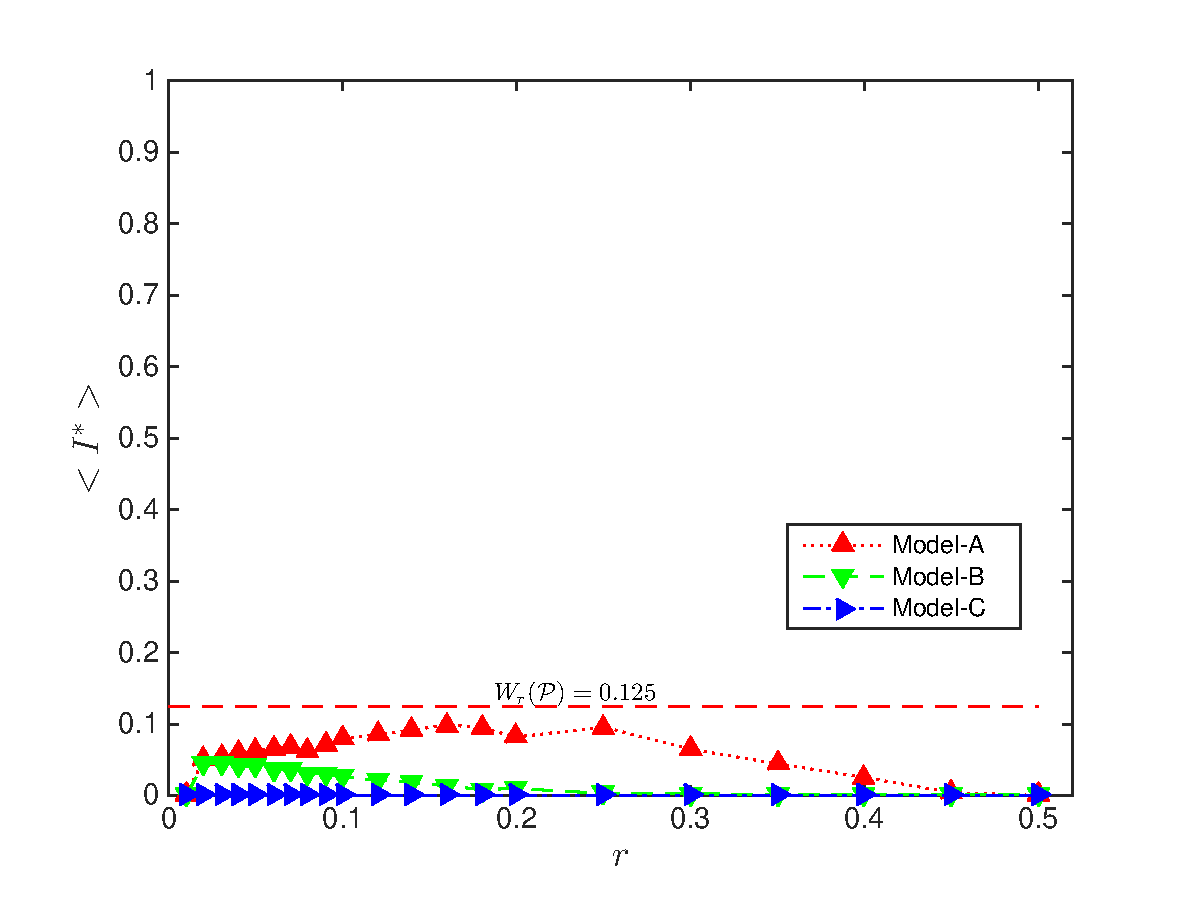
\includegraphics[width=\columnwidth]
			{Fig-FigureA}
		\caption{CaptionA} 
		\label{fig:figureA}
	\end{subfigure}
	\begin{subfigure}{\columnwidth}%
		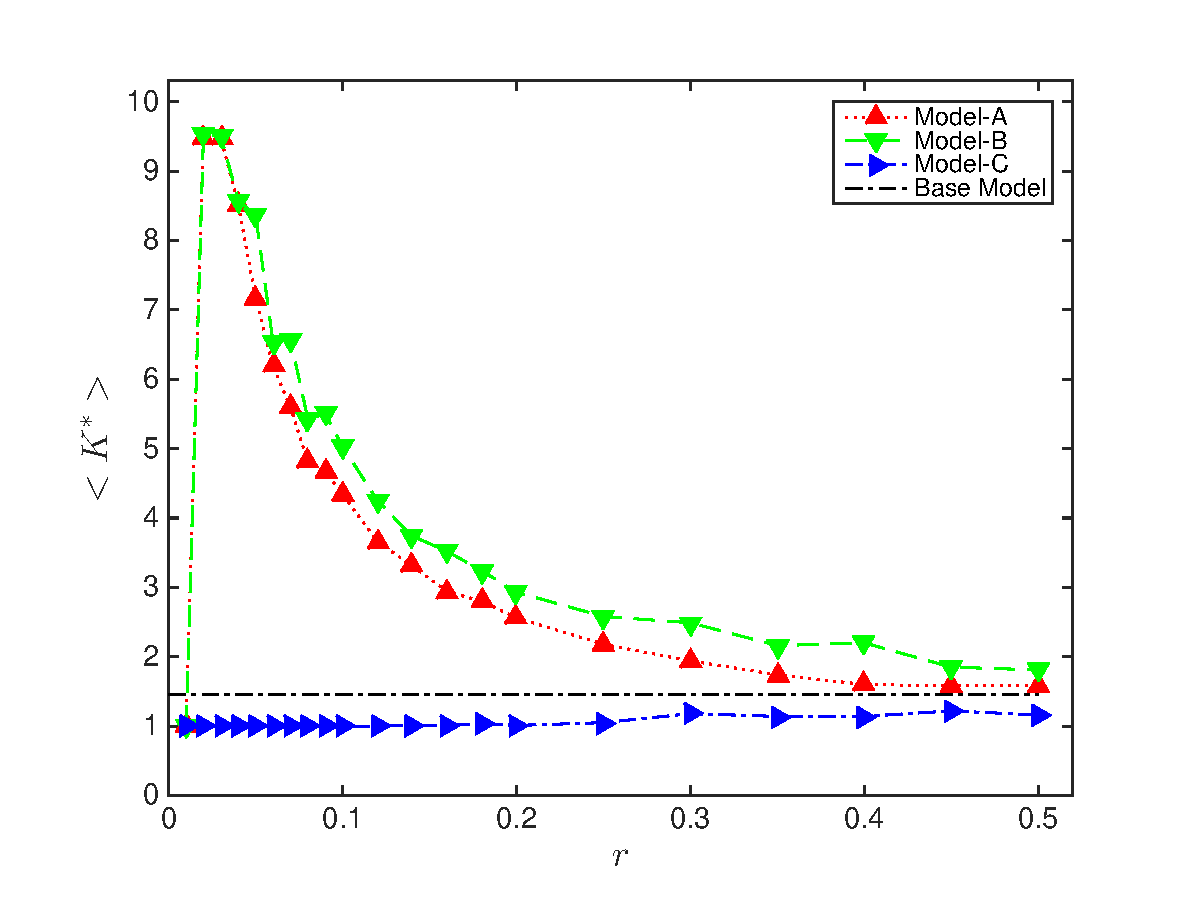
\includegraphics[width=\columnwidth]
			{Fig-FigureB}
		\caption{CaptionB} 
		\label{fig:figureB}
	\end{subfigure}\\
	\begin{subfigure}{\columnwidth}%
		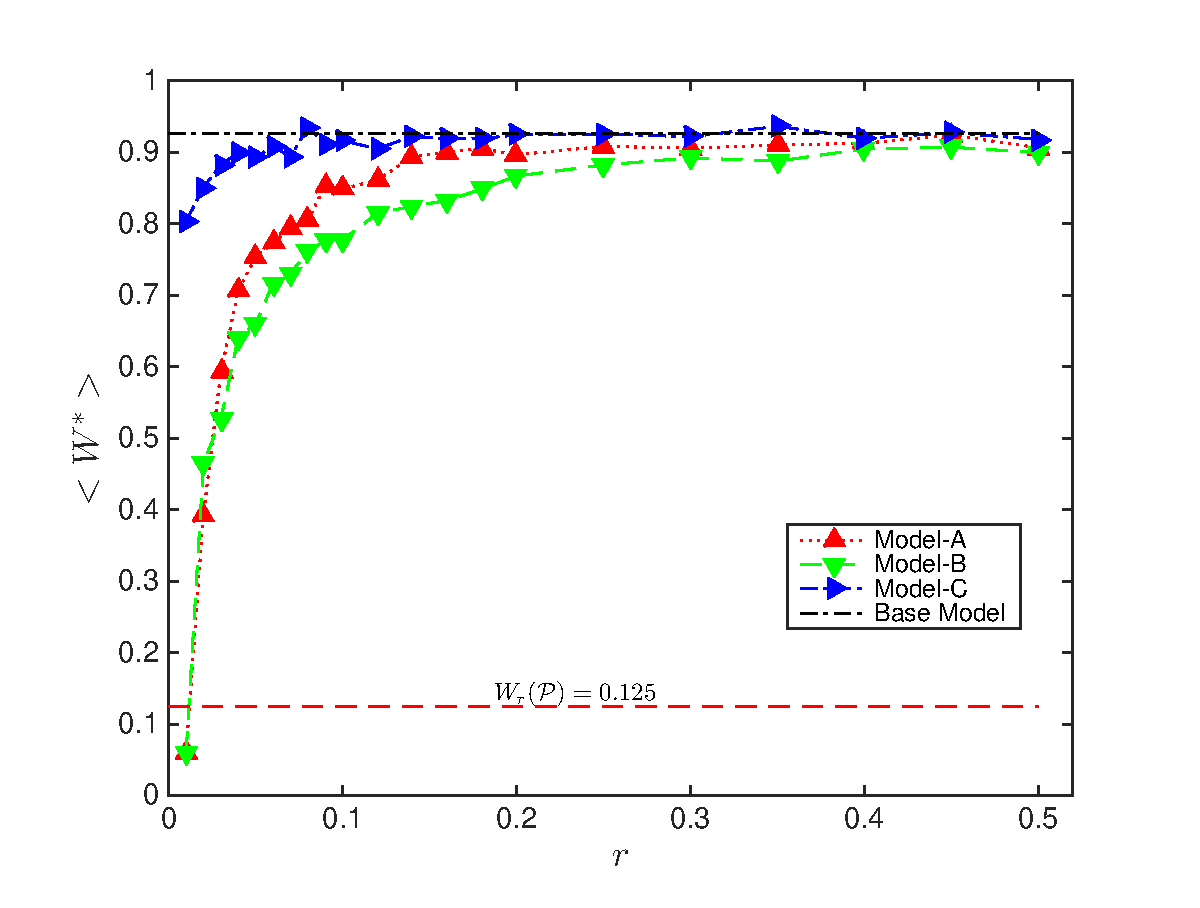
\includegraphics[width=\columnwidth]
			{Fig-FigureC}
		\caption{CaptionC} 
		\label{fig:figureC}
	\end{subfigure}
	\caption{
		Caption of all.
	} % \caption
	\label{fig:oneColumn}
\end{figure}
% +++++++++++++++++++++++++++++++++++++++




% ~~~~~~~~~~~~~~~~~~~~~~~~~~~~~~~~~~~~~~
\subsubsection{Referring figures}

Refer figures using \verb!\reffig!.

It is possible to refer individual subfigures as in 
\reffig{fig:figureB} or
\reffig{fig:figureCin2}
As well as the entire figure as in 
\reffig{fig:oneColumn} or
\reffig{fig:twoColumn}.

% +++++++++++++++++++++++++++++++++++++++
%: -fig 3
\begin{figure*}[!tbp]
	\begin{subfigure}{\columnwidth}%
		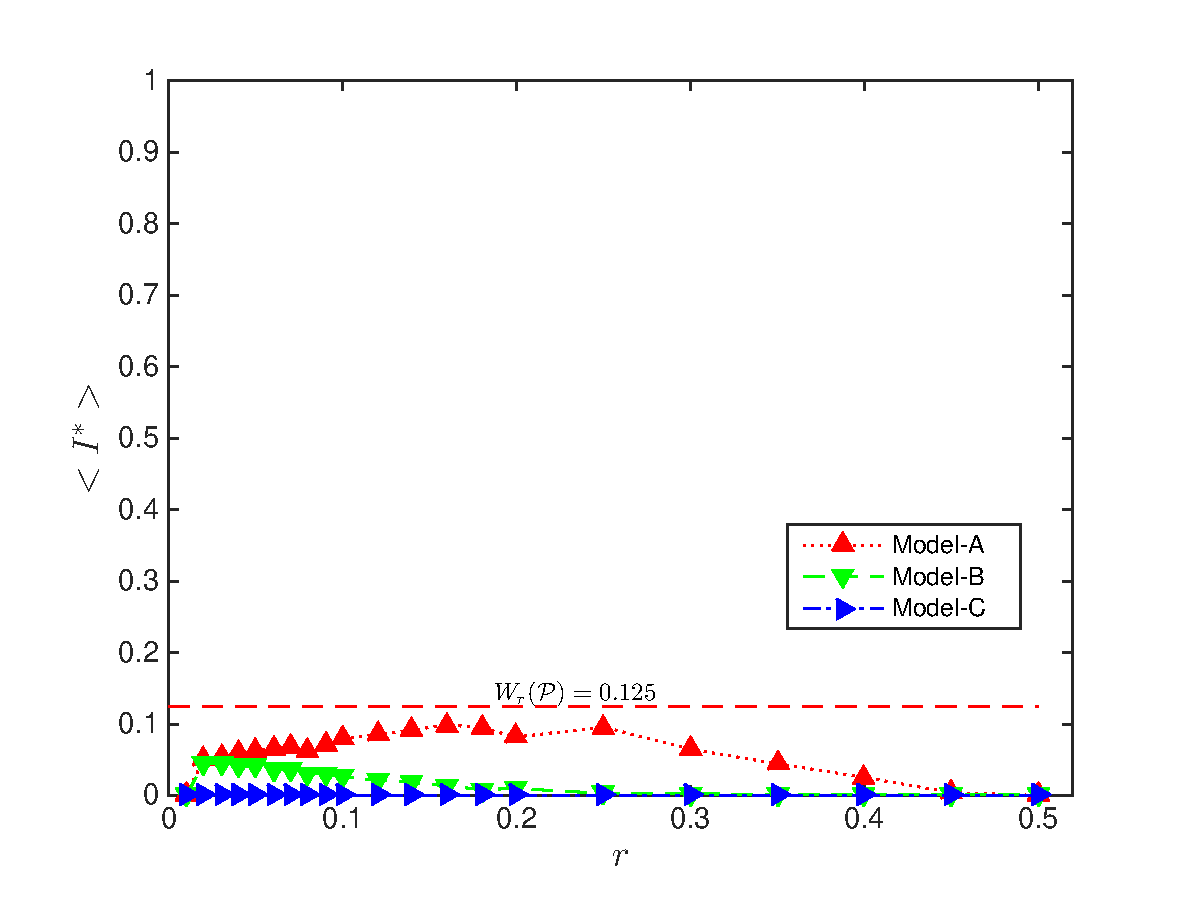
\includegraphics[width=\columnwidth]
			{Fig-FigureA}
		\caption{CaptionA in 2 columns} 
		\label{fig:figureAin2}
	\end{subfigure}
	\begin{subfigure}{\columnwidth}%
		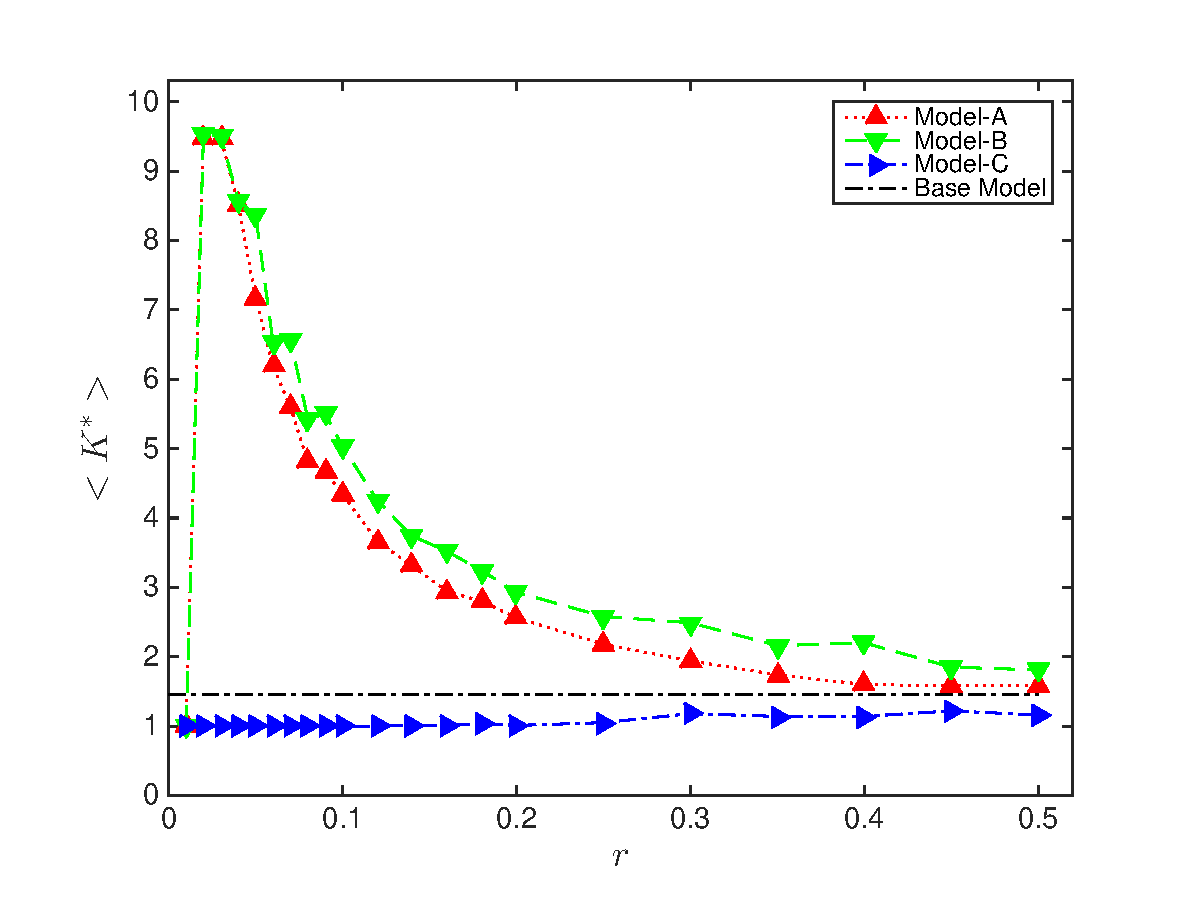
\includegraphics[width=\columnwidth]
			{Fig-FigureB}
		\caption{CaptionB in 2 columns} 
		\label{fig:figureBin2}
	\end{subfigure}\\
	\begin{subfigure}{\columnwidth}%
		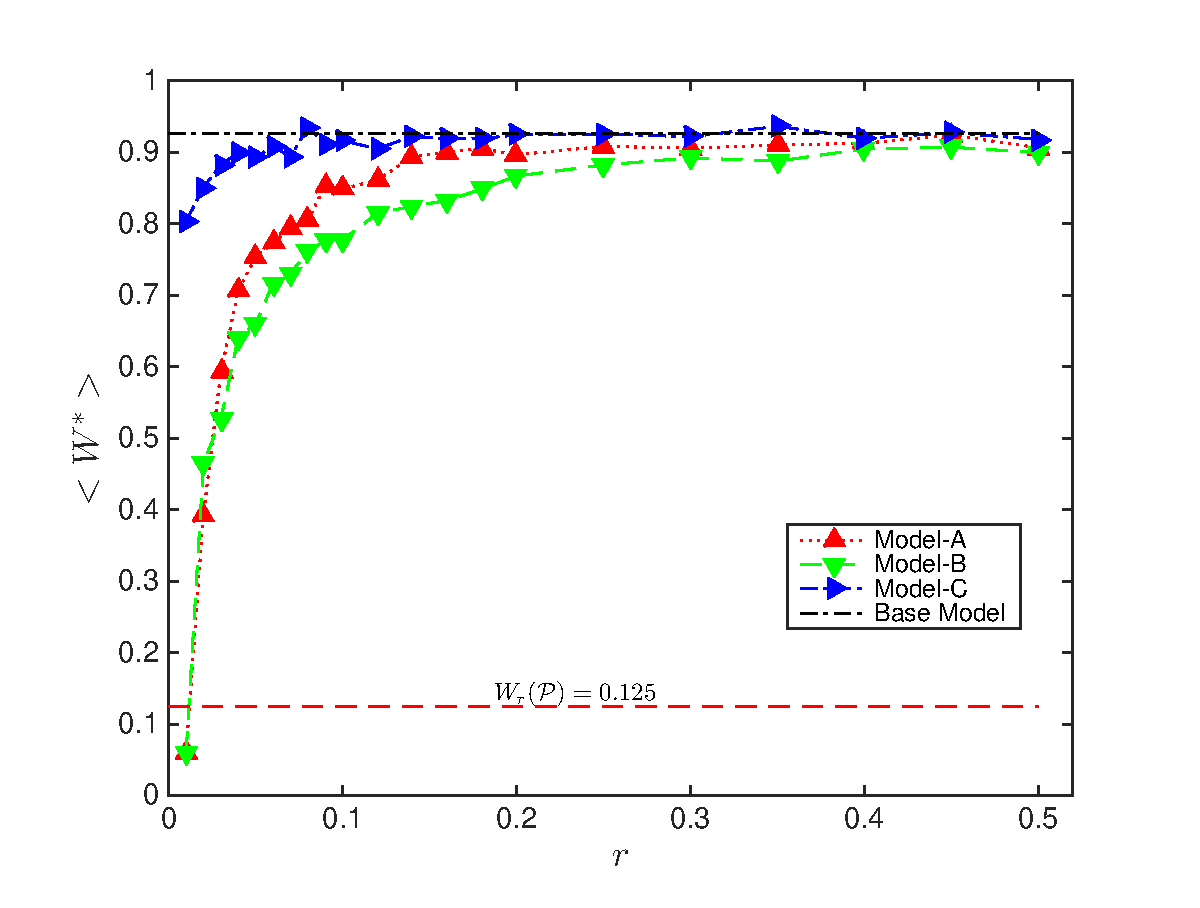
\includegraphics[width=\columnwidth]
			{Fig-FigureC}
		\caption{CaptionC in 2 columns} 
		\label{fig:figureCin2}
	\end{subfigure}
	\caption{
		Figure across two columns.
	} 
	\label{fig:twoColumn}
\end{figure*}
% +++++++++++++++++++++++++++++++++++++++



% ~~~~~~~~~~~~~~~~~~~~~~~~~~~~~~~~~~~~~~
\subsection{Tables}

In tables make sure that numeric column should be right aligned.
Text columns should be left aligned.
Make sure that decimal points in the column are aligned.

% +++++++++++++++++++++++++++++++++++++++ V
%: -table 1
\begin{table}[th]
	\caption{$\gamma$ values for $r > 0.03$}
	\begin{center}
	\begin{tabular}{|r|cc|}
		\hline
		$N$
		&Model-A %\quad
		&Model-B\\
		\hline
		%
		50
		&0.72
		&0.62\\
		%
		100
		&0.69
		&0.63\\
		%
		150
		&0.72
		&0.69\\
		%
		200
		&0.68
		&0.72\\
		\hline
	\end{tabular}
	\end{center}
	\label{tbl:tableA}
\end{table}%
% +++++++++++++++++++++++++++++++++++++++ A




% ~~~~~~~~~~~~~~~~~~~~~~~~~~~~~~~~~~~~~~
\subsubsection{Referring tables}

Refer tables using \verb!\reftbl! as \reftbl{tbl:tableA}.













% ~~~~~~~~~~~~~~~~~~~~~~~~~~~~~~~~~~~~~~=
\section{References}
\label{sec:References}

Journals may have different ways to present references. 
If one uses consistently the same macro for references,
simple change in the macro definition can solve 
the problem of adjusting from the former of one journal to another.
There are a number of objects such as 
definitions ``\refdef{def:PositiveIntegerPowers}'', 
examples ``\refexmp{exp:Generic}'',
figures, 
code listings ``\reflst{lst:QuickStart}''
 that you can refer to.

% ~~~~~~~~~~~~~~~~~~~~~~~~~~~~~~~~~~~~~~=
\begin{thm}[Fundamental theorem of Algebra]
	For all $n \in \hSoN$,
	there is a unique prime factor representation.
	\label{thm:PrimeFactorization}
\end{thm}

% ~~~~~~~~~~~~~~~~~~~~~~~~~~~~~~~~~~~~~~=
\begin{defn}[Positive Integer Powers]
	For all $x \in \hSoX$, and $n \in \hSoN$
	\[
		x^{n} \triangleq
		\begin{cases}
			1, 
			 &n = 0, \\
			x, 
			 &n = 1, \\
			x x^{n-1},
			 &n > 1.
		\end{cases}
	\]
	\label{def:PositiveIntegerPowers}
\end{defn}

% ~~~~~~~~~~~~~~~~~~~~~~~~~~~~~~~~~~~~~~=
\begin{exmp}
	\label{exp:Generic}
	Note that $\hSoX$ is defined in a very generic way.
	We can take $\hSoX$ as 
	natural numbers $\hSoN$,
	real numbers $\hSoR$, or
	$N \times N$ real matrices $\hSoR_{N \times N}$.
\end{exmp}




% ~~~~~~~~~~~~~~~~~~~~~~~~~~~~~~~~~~~~~~=
\subsection{References}

Any object that will be referred,
should have a label declaration such as
\verb!\label{A:B}!,
where 
$A$ is the type indicator and
$B$ is unique label with in the type.
Commonly used type indicator are given in \reftbl{tbl:TypeIndicators}.

% +++++++++++++++++++++++++++++++++++++++
%: -table TypeIndicators
\begin{table}[th]
	\caption{Reference type indicators}
	\begin{center}
	\begin{tabular}{|l |l |l |l |}
		\hline
		Type
		&Indicator
		&Code
		&Result\\
		\hline
		%
		Equation
		&eq
		&\verb!\refeq!
		&\refeq{eq:kBar}\\
		%
		Figure
		&fig
		&\verb!\reffig!
		&\reffig{fig:figureC}\\
		%
		Table
		&tbl
		&\verb!\reftbl!
		&\reftbl{tbl:tableA}\\
		%
		Section
		&sec
		&\verb!\refsec!
		&\refsec{sec:trackChanges}\\
		%
		Citation
		&-
		&\verb!\refcite!
		&\refcite{chomsky1993}\\
		%
		Definition
		&def
		&\verb!\refdef!
		&\refdef{def:PositiveIntegerPowers}\\
		%
		Theorem
		&thm
		&\verb!\refthm!
		&\refthm{thm:PrimeFactorization}\\
		%
		Algorithm
		&alg
		&\verb!\refalg!
		&\refalg{all:quickSort}\\
		%
		List
		&lst
		&\verb!\reflst!
		&\reflst{lst:QuickStart}\\
%		%
%		aaa
%		&aaa
%		&\verb!aaaa!
%		&aaa\\
		\hline
	\end{tabular}
	\end{center}
	\label{tbl:TypeIndicators}
\end{table}%
% +++++++++++++++++++++++++++++++++++++++


It is possible to refer a number of objects within \LaTeX.
Refer an equation \refeq{eq:aij}, which can be obtained by \verb!\refeq{eq:aij}!. 
A figure can be referred by means of \verb!\reffig{fig:oneColumn}!, which produces \reffig{fig:oneColumn}.
Similarly a table can be referred by \reftbl{tbl:tableA} by using \verb!\reftbl{tbl:tableA}!.
A section can be referred by \refsec{sec:trackChanges}, 
that is, 
\verb!\refsec{sec:trackChanges}!.

Refer to a figure as \reffig{fig:Fig-FigureA}.
If you want to refer to a figure with multiple graphs,
there is a way to refer all at once \reffig{fig:oneColumn},
or individually \reffig{fig:figureB} and \reffig{fig:figureC} as required.







% +++++++++++++++++++++++++++++++++++++++ V
%: -List.
\lstinputlisting[language=java,basicstyle=\tiny\ttfamily,label=lst:QuickStart,caption=Code segment]
	{code-sample.java}
% +++++++++++++++++++++++++++++++++++++++ A




% ~~~~~~~~~~~~~~~~~~~~~~~~~~~~~~~~~~~~~~
\section{Citations and BibTeX}

Use citation at  the end of sentence as much as possible.
In this way, 
you can see the citations easily in the text.
Use 
{\footnotesize{\verb!\bibliographystyle{ieeetr}!}
for bibliography,
which provides the title of the cited resource, too. 




% ~~~~~~~~~~~~~~~~~~~~~~~~~~~~~~~~~~~~~~
\subsection{Citing}

Check the source to see how the resources are cited~\cite{%
	chomsky1993,%
%	knuth1984texbook,%
	wikiComplexNetwork}.
This way is much easier for maintenance
when you need to add, remove or commend out any citations.
Some styles organized consecutive citations in a special way,
as here~\cite{%
	feynman1965feynman,
	feynman2018computation,
	feynman2018gravitation,
	feynman1985surely}.
~\refcite{%
	acemoglu2010},
if a sentence starts with citation,
As this one,
start with~\refcite{%
	acemoglu2010}  
not with~\cite{%
	acemoglu2010}.

Always connect citation to the word at the left with \verb!~!, 
i.e., ``tilde'', 
as in the case here~\cite{%
	acemoglu2010}.
This nicely handles the problems occur in the citations happening at the line ends.

In \hCode{.pdf} file, citations are in color and usually acts as a link.
If you want to modify,
see 
\hCode{linkcolor=red}
in 
\hCode{hyperref}.




% ~~~~~~~~~~~~~~~~~~~~~~~~~~~~~~~~~~~~~~
\subsection{BibTeX}

Use \hCode{BibTeX} for managing references.
Use the same file name for both the \hCode{.tex}  file and the \hCode{.bib} file such as
\hCode{aaa.tex} and \hCode{aaa.bib}.
The \hCode{.bib} file is defined at the end of this file with
\hCode{bibliographystyle{IEEEtran}} and
\hCode{bibliography{bibFile}}.

Note that citation process requires four compilations 
(i)~LaTeX, 
(ii)~BibTex, 
(iii)~LaTeX, and  
(iv)~LaTeX,
in this order.




% ~~~~~~~~~~~~~~~~~~~~~~~~~~~~~~~~~~~~~~
\subsubsection{Unsolved problems}

Citing a webpage is an open question for me.
It is suggested to use \hCode{@online} but my system (TeXShop+BibDesk) does not support that.
See
\href
	{https://tex.stackexchange.com/questions/211364/what-is-the-best-way-to-handle-bibliographies-which-include-a-lot-of-online-sour}
	{What is the best way to handle bibliographies which include a lot of online sources?}, 
\href
	{https://tex.stackexchange.com/questions/268433/bibdesk-incompatible-webpage-field}
	{Bibdesk incompatible webpage field}







% ~~~~~~~~~~~~~~~~~~~~~~~~~~~~~~~~~~~~~~
\section{Source Control}
\label{sec:sourceControl}

Consider \LaTeX\ code as programming language code. 
Well,  it is actually a programming language.
Hence use a source control systems such as \hCode{git}.

Please use \hCode{.gitignore} properly so that only the ``source'' files are controlled by \hCode{git}.
Clearly, \hCode{aaa.tex} and \hCode{aaa.bib} are source files.
So does the files used in figures,
such as \hCode{Fig-aaa.eps}.

Make sure that no ``generated'' files, 
such as \hCode{aaa.pdf}, \hCode{aaa.log} generated by \LaTeX, 
go to the git repository.
It is recommended to use \hCode{.gitignore} in 
\href
	{https://github.com/halukbingol/gitignore}
	{https://github.com/halukbingol/gitignore},
which is configured for \LaTeX\ usages as well as some coding such as java.




% ~~~~~~~~~~~~~~~~~~~~~~~~~~~~~~~~~~~~~~
\subsection{Some useful hints}

In order to see the differences between last two commits,
type \hCode{git diff HEAD\^\ HEAD} in the terminal.
It is better to use \hCode{git difftool HEAD\^\ HEAD} 
if your visual diff tool is configured.
See
\href
	{https://stackoverflow.com/questions/9903541/finding-diff-between-current-and-last-version}
	{Finding diff between current and last version}~\cite{%
	stackoverflow0findingDiff}.





% ~~~~~~~~~~~~~~~~~~~~~~~~~~~~~~~~~~~~~~
\section{Multi-Author Case}

Usually more than one author involved.
They have to keep track of changes, leave messages to each other
while the paper developes.

Suppose we have two authors, namely HB and AB.
Note that you need to modify 
\hCode{definechangesauthor}
in 
\hCode{changes} package.
You may want to set different colors, too.



% ~~~~~~~~~~~~~~~~~~~~~~~~~~~~~~~~~~~~~~
\subsection{Track Changes}
\label{sec:trackChanges}

Authors should be able to add, delete and change parts of the document.
\deleted[id=hb]{
	HB removes this part.
}
\added[id=ab]{
	AB adds this part.
}
HB wants to replace some part with some others as
\replaced[id=hb]{
	the new text
}{
	the old text
}

This is \highlight{highlighted} text.
This is \highlight[id=hb]{highlighted} text too.
This is more \highlight[id=hb, comment={Good one.}]{highlighted} text
.
This is the last \highlight[comment=remember]{highlighted} text.

This is \comment{Sure}commented text.
This is \comment[id=hb]{Correct.}commented text too.


% ~~~~~~~~~~~~~~~~~~~~~~~~~~~~~~~~~~~~~~
\subsection{Communicate with Footnotes}

Another way to communicate between authors is to use of footnotes
\hbFootnote{HB}{
	This is a footnote by HB.
}.
The other author has another footnote
\hbFootnote{AB}{
	This is a footnote by AB.
}
.
Note that this is not the same as regular footnotes that you intent to keep in your final document such as~\footnote{
	This is a footnote that should stay in the final version of the document.
}.
These communication footnotes should be removed at the end of development process.
Color of ``@HB'' at the start of the footnote should warn you, if you are looking the \hbDPdf\ file online.
One final search in the \hbDTex\ file for ``@'' should help you to locate unremoved ones.




% ~~~~~~~~~~~~~~~~~~~~~~~~~~~~~~~~~~~~~~=
\section{Math}

Please see \LaTeX\ cheat sheet available at
\href
	{https://github.com/halukbingol/zintCheatSheet-LaTeX-DiscreteMath}
	{https://github.com/halukbingol/zintCheatSheet-LaTeX-DiscreteMath}
for many \LaTeX\ tricks.

Please note the usage of spaces while writing math in \hbDTex\ file.
Proper usage of space will improve readability of your \LaTeX\ code.




% ~~~~~~~~~~~~~~~~~~~~~~~~~~~~~~~~~~~~~~
\subsection{Math in-line mode}

This is math ``in-line'' mode,
i.e., math with in the lines of text. 
There are two ways to switch to in-line math mode.
Use \verb!\( ... \)!, which is the \LaTeX\ way, and
\verb!$ ... $!, which is the \TeX\ way.
These are examples of in-line math usages.
The row sum of row $i$ is given as
$
	s_{i} = \sum_{j=1}^{N} a_{i j}
$,
where $\mathbf{A} = [a_{i j}]$ is a matrix.
One more example is
\(
	e_{\mu x} 
	= \frac{a_{\mu x}}{\sum_{x'=1}^{S} a_{\mu x'}},
\)
and
\(
	d_{x \mu} 
	= \frac{a_{\mu x}}{\sum_{\mu'=1}^{M} a_{\mu'x}}.
\)




% ~~~~~~~~~~~~~~~~~~~~~~~~~~~~~~~~~~~~~~
\subsection{Math in display mode}

If you want your math in ``display'' mode there are two options. 
If you are not going to refer the equation again, 
use \verb!\[ ... \]!.
This is the same example in display mode
\[
	e_{\mu x} 
	= \frac{a_{\mu x}}{\sum_{x'=1}^{S} a_{\mu x'}},
	\quad
	d_{x \mu} 
	= \frac{a_{\mu x}}{\sum_{\mu'=1}^{M} a_{\mu'x}}.
\]
Note the usage of \verb!\quad! to separate the two.

If you are going to refer the equation in the text,
then it should be numbered.
To do that,
use \verb!\begin{align} ... \end{align}! to obtain
\begin{align}
	a_{ij} =
		\frac{1}{M}
		\sum_{\mu = 1}^{M} 
		{\sum_{x = 1}^{S} 
			e_{\mu x}^{(i)}
			d_{x \mu}^{(j)} }.
	\label{eq:aij}
\end{align}




% ~~~~~~~~~~~~~~~~~~~~~~~~~~~~~~~~~~~~~~
\subsection{Multi-line equations}

If you have multiple line derivation,
then \hCode{align} block with \verb!&! is the solution.
\begin{align}
	a 
	&= bbbbb\\
	&= cccc \label{eq:cccc}\\
	&= ddd.
\end{align}
Note that each line has a number that can be referred.

If you do not refer the equation later,
get rid off numbers by using \hCode{align*} block.
as
\begin{align*}
	a 
	&= bbbbb\\
	&= cccc\\
	&= ddd.
\end{align*}

It is possible to explain how you move from one line to the next as 
\begin{align*}
	a 
	&= bbbbb
		&\text{ because } x = 5\\
	&= cccc
		&\text{ side $AB$ intersects side $BC$}\\
	&= ddd.
\end{align*}




% ~~~~~~~~~~~~~~~~~~~~~~~~~~~~~~~~~~~~~~
\subsubsection{Referring to equations}

Refer equations using \verb!\refeq! as \refeq{eq:aij}.
It is possible to refer a line in a multiple line derivation as \refeq{eq:cccc}.
You can refer to an equation \refeq{eq:equationInAppendix} in the appendix, too.




% ~~~~~~~~~~~~~~~~~~~~~~~~~~~~~~~~~~~~~~
\subsection{Subscripts and superscripts}

Always use curly brackets when you use subscripts or superscripts 
even if there is no need due to single symbol.
For example \verb!a_{i}! is better than \verb!a_i! 
if you consider
\verb!a_{ij}! and \verb!a_ij!.
They produce
$a_{i}$,
$a_i$,
$a_{ij}$, and 
$a_ij$,
respectively.




% ~~~~~~~~~~~~~~~~~~~~~~~~~~~~~~~~~~~~~~=
\subsubsection{Some examples}

\[
	\sum_{x = 1}^{S} 
		e_{\mu x}^{(i)}
		d_{x \mu}^{(j)} 
\]
\[
	A= 	
	\frac
		{1}
		{2 {\hAbs{\mathcal{C}} \choose 2}} 
	\sum_{i \in \mathcal{C}}
	\sum_{
		\substack{
			j \in \mathcal{C}\\
			j \neq i
		}
	} 
	b_{ij}.
\]
\[
	\hat{K} =
		\hArgmax
			{K}
			{{\mathbb{P}_{K}}}.
\]




% ~~~~~~~~~~~~~~~~~~~~~~~~~~~~~~~~~~~~~~~ 
\section*{Acknowledgments}

%\textbf{Acknowledgments.}
This work is partially supported by 
the Turkish Directorate of Strategy and Budget
under the TAM Project number 2007K12-873.





% ~~~~~~~~~~~~~~~~~~~~~~~~~~~~~~~~~~~~~~
\appendix
%: ==== HB Header Common for Appendix v20170517 ====V
\newcommand{\hbAppendixPrefix}{A}
%
\renewcommand{\thefigure}{\hbAppendixPrefix\arabic{figure}}
\setcounter{figure}{0}
\renewcommand{\thetable}{\hbAppendixPrefix\arabic{table}} 
\setcounter{table}{0}
\renewcommand{\theequation}{\hbAppendixPrefix\arabic{equation}} 
\setcounter{equation}{0}
% ==== HB Header Common for Appendix v20170517 ====A




% ~~~~~~~~~~~~~~~~~~~~~~~~~~~~~~~~~~~~~~
\section{Dummy appendix item}
	\label{sec:dummyAppendix}

%\lipsum[1-1]

This is an equation
\begin{equation}
	\label{eq:equationInAppendix}
	\bar{k} = \hArgmin{k} d(\mathbf{x}_{n},  \mathbf{m}_{k}(t-1)),
\end{equation}
which will be referred else where.




% ~~~~~~~~~~~~~~~~~~~~~~~~~~~~~~~~~~~~~~
\section{Header Part}

Note that timestamp \hbTimeStamp\ that helps to keep track of versions 
while the paper is being developed.
Do not forget to remove it before submission.





% ~~~~~~~~~~~~~~~~~~~~~~~~~~~~~~~~~~~~~~
\subsection{Common Packages}

Common packages are listed.




% ~~~~~~~~~~~~~~~~~~~~~~~~~~~~~~~~~~~~~~
\subsection{Common Declarations}

Common and frequently used macros are defined.




% ~~~~~~~~~~~~~~~~~~~~~~~~~~~~~~~~~~~~~~
\subsection{Specific}

Anything that is specific to this paper should be defined in \hbSSpecific\ in the header.




% ~~~~~~~~~~~~~~~~~~~~~~~~~~~~~~~~~~~~~~
\section{TexShop Specific}

I use TexShop.
It has some features that I use.
\begin{itemize}

	\item
	Tag list feature of TeXShop enables you to directly go to a segment of your document.
	Sections are automatically listed in here.
	I need to extend that for my purposes.
	A \LaTeX\  comment starts with ``\hCode{\%}''.
	If comment starts with`` \hCode{\%:}'',
	note the additional ``\hCode{:}'',
	then it is listed in the tags list, too.
	I use this feature to fast access to some parts of the document such as figures and tables.
	So I add comments such as 
	``\hCode{\%: -fig.1}'' for figure 1 and
	``\hCode{\%: -tbl 3}'' for table 3.
	
	\item 
	\hCode{\% !TEX spellcheck = en\_US} forces the spellchecker to use American English.
	
\end{itemize}




% ~~~~~~~~~~~~~~~~~~~~~~~~~~~~~~~~~~~~~~=
%\DeclareBibliographyAlias{webpage}{online}
%https://tex.stackexchange.com/questions/268433/bibdesk-incompatible-webpage-field
\bibliographystyle{ieeetr}

\bibliography{bingol-MyLaTeXBestPractices}



% =========
\listofchanges   % track changes use at the bottom
% =========



\end{document}






